\section{LBM Algorithm}\label{algoritmus LBM}
The LBM algorithm can be summarized in several steps:
\begin{enumerate}
	\item \textbf{Initialization} of initial conditions on the grid, discussed in section \ref{pocatecni a okrajove podminky}.
	\item \textbf{Cycle} ending with the fulfillment of a user-specified termination condition.
	\begin{enumerate}
		\item \textbf{Streaming} of post-collision distribution functions \( f^{*}_{k} \) in the respective directions \( \vec{\xi_{k}} \).
		\item \textbf{Calculation of macroscopic quantities} using the relations \eqref{macroeq}.
		\item \textbf{Collision}, where the post-collision state of the distribution function is calculated using \eqref{eq:collision}, and \textbf{application of boundary conditions}, discussed in section \ref{pocatecni a okrajove podminky}.
	\end{enumerate}
	\item \textbf{End of the algorithm.}
\end{enumerate}
A flowchart of the LBM algorithm is shown in Figure \ref{fig:algo}.
\begin{figure}[h]
	\centering
	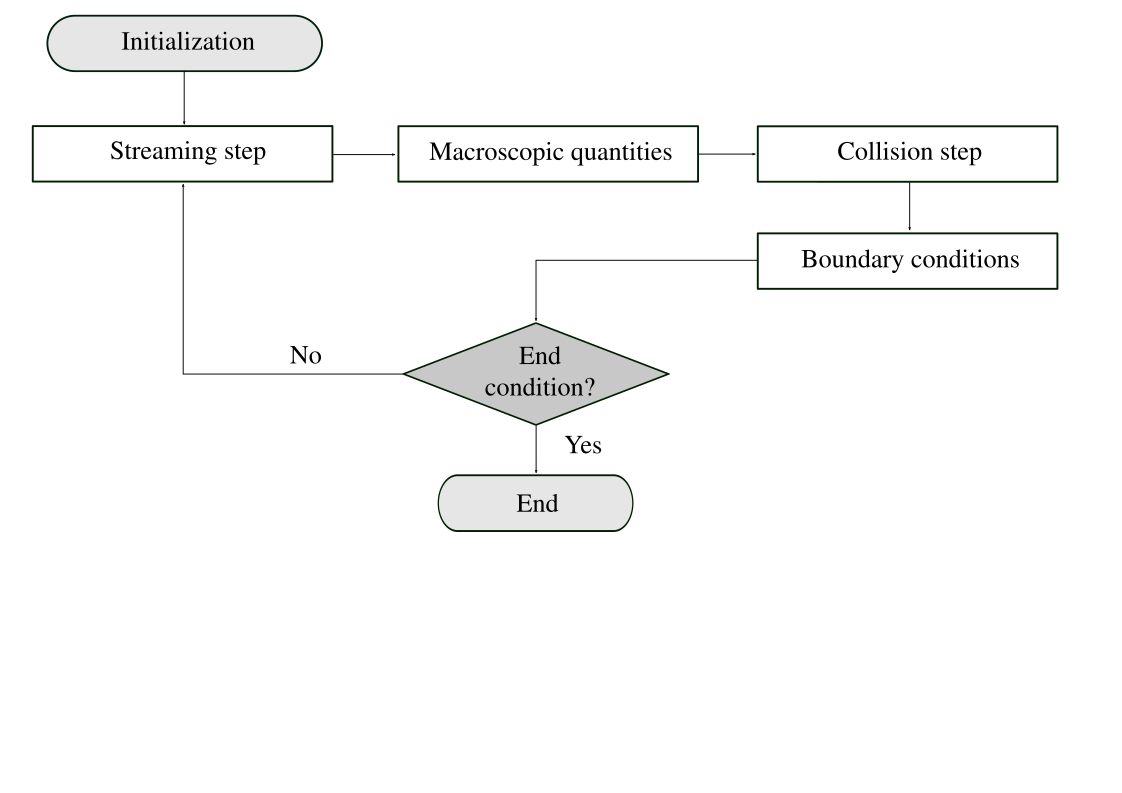
\includegraphics[width=0.78\textwidth]{figures/algo-bw.pdf}
	\caption{Flowchart of the LBM algorithm.}
	\label{fig:algo}
\end{figure}